\section{Lecture 15: Discrete time signal processing system}


\subsection{Introduction}
In this lecture, we will see how we can take all the processing that we wish to do on continuous-time signals into the discrete-time domain. This can be easily done on a computer.

\subsection{General Discrete-time processing}
We will be dealing with continuous signals which have a Fourier transform and systems which have a frequency response. From our previous discussions on sampling and reconstruction, we know that we need continuous signals to be \textit{band-limited} if we wish to perfectly reconstruct them after sampling. Hence we will limit ourselves to those continuous-time signals whose Fourier transform is zero beyond $|\Omega| \geq \Omega_{m}$. 

Recall that every type of sampling ultimately means that there is a repetition of the the spectrum of the original signal at every integral multiple of the sampling frequency. The sampling frequency has to be \textit{greater} than twice the maximum frequency at which the signal is non-zero (in order to have no aliasing or overlap between any two carbon copies of the original spectrum). That is, $f_{s} > 2\frac{\Omega_{m}}{2\pi}$. This is the \textit{analog-to-digital conversion}. From Nyquist's principle, it is then possible to perfectly reconstruct the signal from its samples. This is called \textit{digital-to-analog conversion}. 

But there is no purpose to simply sampling and reconstructing. The beauty in this scheme is when we process the samples i.e when we do something between the analog-to-digital conversion and digital-to-analog conversion. This is called discrete-time signal processing (DSP). As we will be dealing with band-limited signals, it is enough to restrict the discrete-time systems also to this band. 

Let the input band-limited signal have a Fourier transform $X(\Omega)$ and the output signal have a Fourier transform $Y(\Omega)$. If the frequency response of the LSI system is $H(\Omega)$, then we have $Y(\Omega) = X(\Omega)H(\Omega)$. Let us look at a consequence of this in Fig. \ref{conseq}. 
\begin{figure}[h] 
        \centering
        
                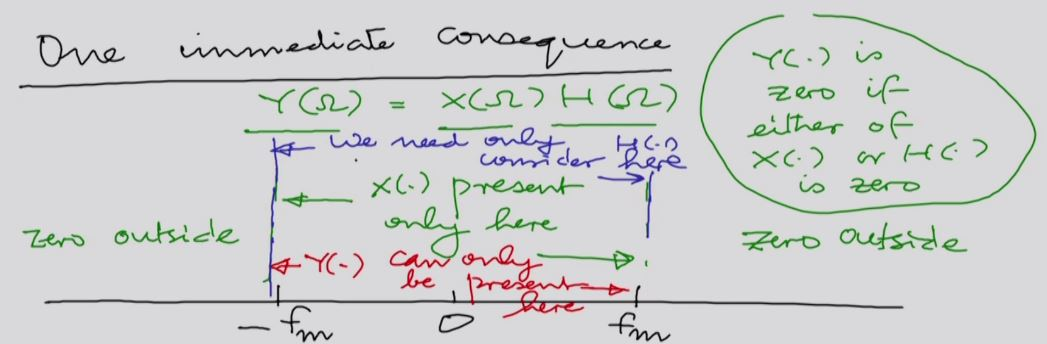
\includegraphics[width=\textwidth]{conseq.JPG}
                \caption{Region of relevance for $Y(\Omega)$ and $H(\Omega)$}
                \label{conseq}
        
\end{figure}
Because of the previous relation, $Y(\Omega)$ is zero whenever $X(\Omega)$ or $H(\Omega)$ is zero. Hence because of the band-limited nature of $X(\Omega)$, we can ascertain that $Y(\Omega)$ is also band-limited between $-\Omega_{m}$ and $\Omega_{m}$. As a consequence, we need consider $H(\Omega)$ in the same band (shown in blue in Fig.\ref{conseq}). 



\subsection{Going from continuous-time to discrete-time signal processing}
A discrete-time signal processing system does the following:
\begin{enumerate}
\item It takes a continuous-time band-limited signal $x(t)$, band-limited as $-\Omega_{m} \leq \Omega \leq \Omega_{m}$
\item It samples it at a rate $f_{s}$, which as per the Nyquist principle has to be \textit{greater} than $2\frac{\Omega_{m}}{2\pi}$ which yields the input sequence $x[nT_{s}]$. For convenience, we denote this as $x[n]$ by calling $T_{s}$ as the unit time. This is called as \textit{normalisation}.
\item This input sequence $x[n]$ is fed into a linear shift-invariant system with the impulse response $h[n]$, to yield the output sequence $y[n]$.  
\end{enumerate}

Our aim is to process a continuous-time signal $x(t)$ by operating a system (frequency response = $H(\Omega)$) on it. We want to devise a discrete-time system which can achieve the same effect when we operate it on $x[n]$ and reconstruct the resulting $y[n]$. Let us look at this in more detail.
\\

We have a continuous-time band-limited signal $x(t)$. We operate (process) a continuous-time LSI system with frequency response $H(\Omega)$, to obtain $y(t)$. The output signal has to be band-limited. We are quite safe if we restrict $H(\Omega)$ to $-\Omega_{m} \leq \Omega \leq \Omega_{m}$. This gives us the discrete system that we are looking for. In other words, we can treat the restricted version of the frequency response of $H(\Omega)$ as the frequency response of the discrete-time system. 

{\bf Important!}- The discrete-time Fourier transform of $h[n]$, $H(\omega)$ is essentially the continuous-time Fourier transform of $h(t)$ restricted between $-\Omega_{m}$ and $\Omega_{m}$ and then normalised. 

\subsection{Graphical view of restriction and normalisation of $H(\Omega)$}
\subsubsection{Restriction}
\begin{figure}[h] 
        \centering
        
                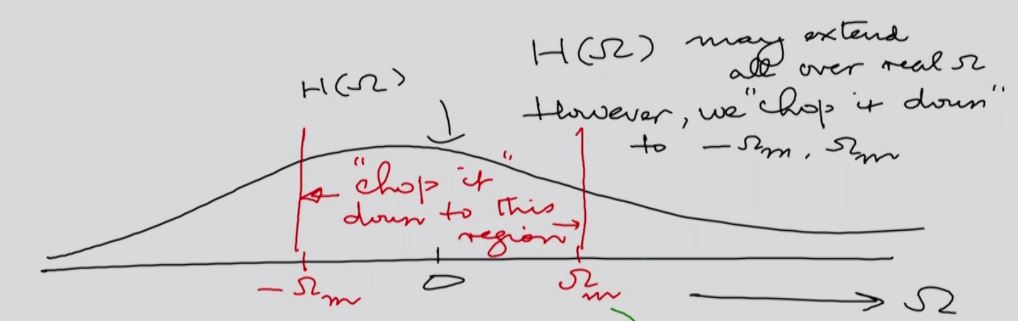
\includegraphics[width=\textwidth]{chopping.JPG}
                \caption{Restriction on the frequency axis}
                \label{chopping}
        
\end{figure}

\subsubsection{Normalisation}
Let us sample the signal at the frequency $\Omega_{s}$ such that $\Omega_{s} > 2 \Omega_{m}$. Hence instead of restricting $H(\Omega)$ only to $\Omega_{m}$, it would be better if we restrict it to $\Omega_{s}/2$, in order to include many more band-limited signals. Hence we normalise $\Omega_{s}/2$ to $\pi$ and $-\Omega_{s}/2$ to $-\pi$. 
\begin{figure}[h] 
        \centering
        
                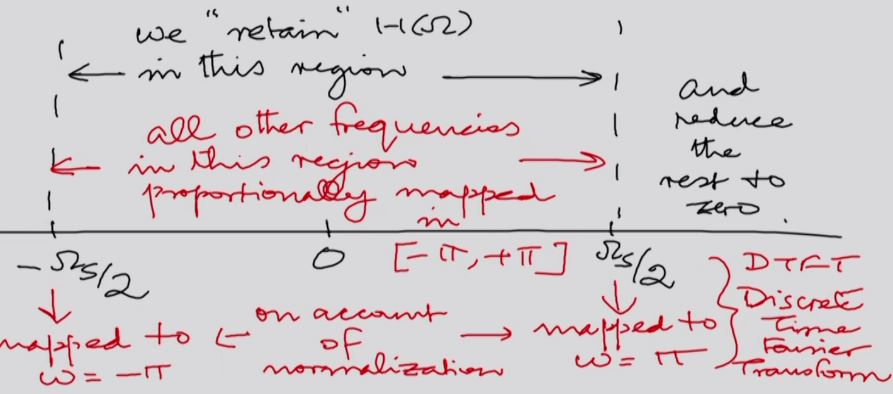
\includegraphics[width=\textwidth]{normalise.JPG}
                \caption{Normalisation of the frequency axis with respect to sampling frequency}
                \label{normalise}
        
\end{figure}
Now we obtain the discrete-time Fourier transform $H(\omega)$ of the desired discrete-time system.
\\

The whole process of DSP of the equivalent continuous-time counterparts, can now be summarised in Fig.\ref{whole}. 
\begin{figure}[h] 
        \centering
        
                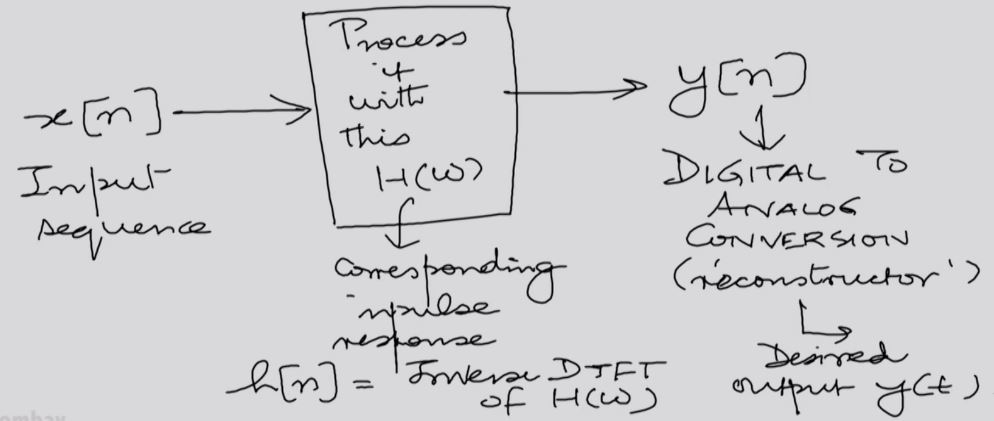
\includegraphics[width=\textwidth]{whole.JPG}
                \caption{Digital equivalent of the continuous-time signal processing}
                \label{whole}
        
\end{figure}

\subsection{Example of Constructing a Discrete-Time System Equivalent to an RC Filter}
Let the problem be as shown in Fig.\ref{problem}. 
\begin{figure}[h]
        \centering
        
                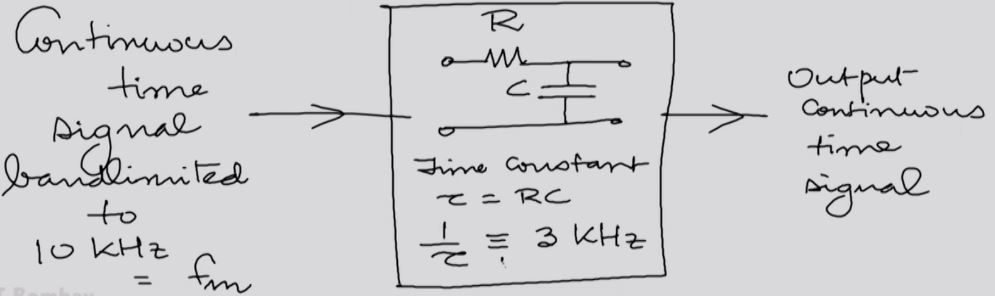
\includegraphics[width=\textwidth]{problem.JPG}
                \caption{Continuous-time processing that we wish to do}
                \label{problem}
        
\end{figure}
We want to pass a signal band-limited to 10kHz through an RC filter (low-pass) with a time constant 'equivalent' to 3kHz.

In order to find the equivalent discrete-time system, we need to know the frequency response of the continuous-time system. So let us find the frequency response of the system, the RC filter given in Fig.\ref{rcfilter}.  
\begin{figure}[h] 
        \centering
        
                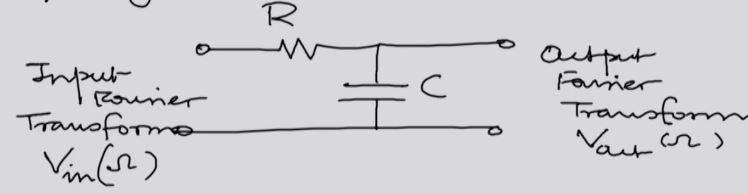
\includegraphics[width=\textwidth]{rcfilter.JPG}
                \caption{Frequency response of RC filter}
                \label{rcfilter}
        
\end{figure}
The impedence of the capacitor at a frequency of $\Omega$ is $\frac{1}{j\Omega C}$. From voltage divider principle,
\begin{equation}
\begin{split}
\frac{V_{out}(\Omega)}{V_{in}(\Omega)} & = \frac{\frac{1}{j\Omega C}}{R + \frac{1}{j\Omega C}}\\
									   & = \frac{1}{1 + jRC\Omega}\\
                                       & = \frac{1}{1 + j\tau\Omega}
\end{split}
\end{equation}
The frequency response has a magnitude of $\frac{1}{\sqrt{{1 + \tau^{2}\Omega^{2}}}}$. 

\subsection{Significance of certain frequencies}

\subsubsection{Half-power frequency}
At $\Omega = \frac{1}{\tau}$, the magnitude of the ratio of output to input becomes

\begin{equation}
\begin{split}
|H(\frac{1}{\tau})| & = \frac{1}{\sqrt{{1 + 1}}}\\
									   & = \frac{1}{\sqrt{2}}
\end{split}
\end{equation}
Power is proportional to the voltage squared. Hence the power in the output sinusoid at angular frequency $\frac{1}{\tau}$ is \textit{half} that of the power in the input sinusoid. 
\subsubsection{$K$-powerpoint frequency}
The frequency at which the power falls to $K$ times the input power is given by,
\begin{equation}
\begin{split}
|H(\Omega)|^{2} & = \frac{1}{{1 + \tau^{2}\Omega^{2}}}  = K\\
\frac{1}{1 + \tau^{2}\Omega^{2}} & = K\\
1 + \tau^{2}\Omega^{2} & = \frac{1}{K}\\
\Omega^{2} & = \frac{1}{\tau^{2}}(\frac{1}{K} - 1)\\
\Omega & = \sqrt{\frac{1}{\tau^{2}}(\frac{1}{K} - 1)}\\
\Omega & = \frac{1}{\tau}\sqrt{(\frac{1}{K} - 1)}
\end{split}
\end{equation}

If $K$ is 0.1, we fall to 10\% of the input power. The frequency at which this happens,
\begin{equation}
\begin{split}
\Omega & = \frac{1}{\tau}\sqrt{(\frac{1}{0.1} - 1)}\\
       & = \frac{3}{\tau}
\end{split}
\end{equation}

This is why we said earlier that $\frac{1}{\tau}$ is 'equivalent' to 3kHz. It has to be equal to the corresponding angular frequency and not the cycles/second frequency. Therefore, $\frac{1}{\tau} = 2\pi 3$ kHz. Therefore, the RC filter is a low-pass filter where at 9kHz (cycles/sec frequency), the power falls to 10\%; at 3kHz, it falls to 50\% and so on. 

\subsection{Description of the equivalent discrete-time RC filtering process}
As the input signal is band-limited to 10kHz, we have to sample at a frequency greater than 20kHz, say 24kHz. From normalisation, we have that $2\pi12$ kHz corresponds to $\pi$ on the $\omega$ axis. Hence we need to consider the frequency response of the RC-filter also only upto $2\pi12$ kHz as shown in Fig. \ref{truncate}.
\begin{figure}[h] 
        \centering
        
                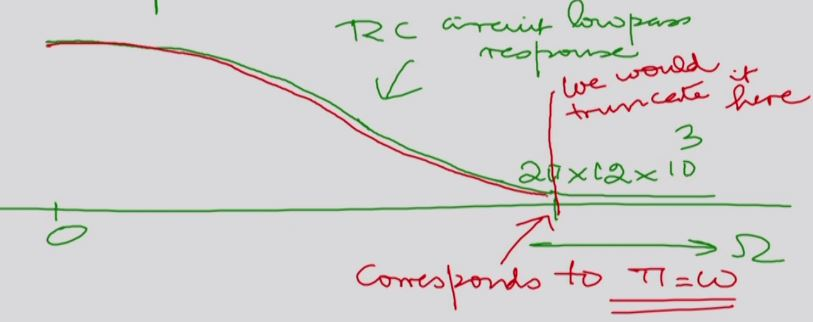
\includegraphics[width=0.7\textwidth]{truncate.JPG}
                \caption{Truncated frequency response to obtain the discrete-time frequency response}
                \label{truncate}
        
\end{figure}
So the frequency of the discrete-time filter would be,
\begin{equation}
\begin{split}
H(\omega) & = \frac{1}{1 + j\tau\Omega}\\
\end{split}
\end{equation}
with the $\Omega$ normalised as following. As $\frac{\Omega_{s}}{2}$ corresponds to $\omega = \pi$, $\Omega$ corresponds to,
\begin{equation}
\begin{split}
\omega & = \Omega\frac{2\pi}{\Omega_{s}}\\
        & = \frac{\Omega}{f_{s}} \\   
        & = \Omega T_{s}
\end{split}
\end{equation}
Therefore, $\Omega = \frac{\omega}{T_{s}}$. Hence,
\begin{equation}
H(\omega)  = \frac{1}{1 + j\tau\frac{\omega}{T_{s}}}
\end{equation}
After normalisation, we have to restrict $\omega$ between $-\pi$ and $\pi$. Also recall that since $H(\omega)$ is a discrete-time Fourier transform, it is periodic with period $2\pi$. Therefore, periodically repeat the frequency response to obtain the full frequency response of the desired discrete-time system. 
\begin{figure}[h] 
        \centering
        
                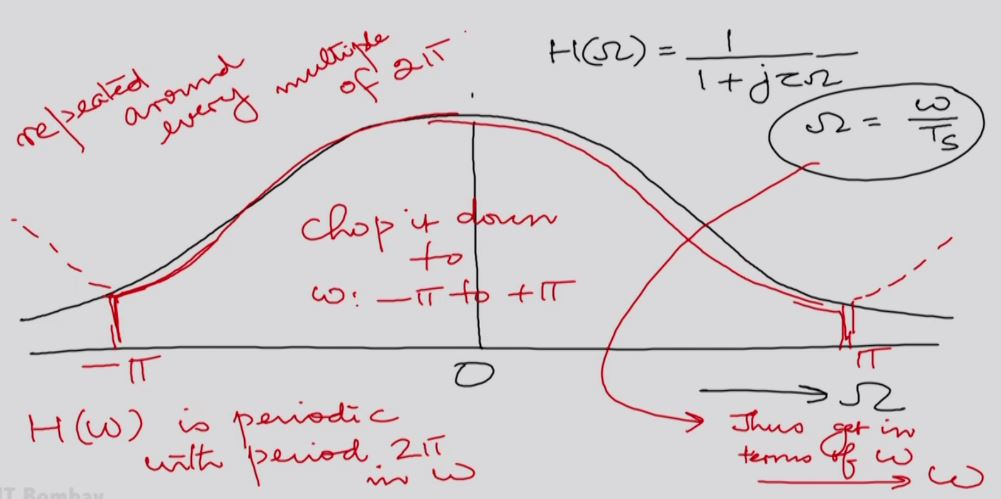
\includegraphics[width=0.7\textwidth]{periodic.JPG}
                \caption{Normalised, restricted and periodically extrapolate the continuous-time frequency response to obtain the discrete-time frequency response}
                \label{periodic}
        
\end{figure}
We can, in principle, find the impulse response $h[n]$ by taking the inverse DTFT of $H(\omega)$, which would be complicated. We can, on the other hand, make an approximation. We could think of the filter as an ideal low-pass filter where $\Omega = \frac{3}{\tau} = 9$ kHz is in the stop-band and $\Omega = \frac{1}{\tau} = 3$ kHz is in the pass-band. We can choose the cut-off frequency to be somewhere in between (say, 6kHz) and treat it as an almost ideal low-pass filter for convenience of calculations. 


